\subsection{Redundancy Checker}
\label{sec:redundant}

We will compare the computation of different iterations
from one loop instance and that of different loop instances from 
one static loop,
and judge whether there is redundancy.
Specifically, several questions need to be answered.

\emph{What to compare?}
Given two loop iterations (or loop instances) $c_1$ and $c_2$, since they 
originate from the same source code $C$, 
a naive approach is to record and compare the value read by
every memory read instruction in $c_1$ and $c_2$. 
%We will know whether $c_1$ and $c_2$ are redundant with each other by comparing
%these values.
We could do better by checking fewer instructions, as
some of these values are determined by values read earlier in $c_1$ and
$c_2$. Informally speaking, we only need to compare \textit{input}
values of $c_1$ and $c_2$ to decide whether they are redundant with each other. 
We will present formal definition of \textit{input} and the detailed algorithms
in Section \ref{sec:dependence}.

%TODO
%Among the the above two potential solutions, our design chooses the second one,
%because it is
%more informative for performance diagnosis 
%to track the cause rather than the effect.

\emph{How to compare?}
Naively, we can judge two iterations or two
loop instances to be redundant with each other only when they read exactly
the same data and conduct exactly the same computation. However,
in practice, redundant loops may be doing largely, but not completely,
the same computation across iterations or loop instances. 
%It is also possible
%TODO define loop instance.
%that only some, instead of all, iterations in a loop are doing redundant
%computation. 
We will discuss how we handle this issue in Section \ref{sec:cal}.



\emph{How to lower the overhead of record-and-compare?}
We will use both static optimization 
(Section \ref{sec:perf})
and dynamic sampling (Section \ref{sec:inst})
to reduce the amount of data that is recorded and compared, reducing
time and spatial overhead.
%TODO static analysis alone is not sufficient, because some redundant is
%workload dependent

\subsubsection{Identifying and recording \textit{inputs}}
\label{sec:dependence}

Informally, we use static analysis to identify a set of 
memory-read instructions that the computation of code $C$
depends on. We refer
to these instructions as \textit{input instructions} for $C$. 
The values returned
from them at run-time, referred to as \textit{inputs}, 
will be tracked and compared to identify
redundant computation among different instances of $C$.

Specifically, \Tool first identifies side-effect instructions in $C$,
similar with that in Section \ref{sec:s_workless}. 
It then conducts 
backward static slicing 
from these instructions, considering control and data
dependency. For every memory read $r$ 
(\texttt{read(v)}) that static slicing encounters, \Tool checks whether $r$
satisfies either one of the following two conditions. 
If $r$ does, it is marked as
an \textit{input} instruction; otherwise, \Tool continues growing the
slice beyond $r$.
The two conditions are:
(1) the value of $v$ is defined outside $C$;
(2) $v$ is a heap or global variable.
The rationale for the first condition is that slicing outside $C$ is
unnecessary for redundancy judgement among instances of $C$.
The rationale for the second condition is that tracking data-dependency
through heap or global variables is complicated in multi-threaded C/C++
programs.
The analysis for cross-iteration and cross-loop redundancy analysis is similar
--- simply replacing $C$ in the above algorithm with one iteration or
the whole loop body.

%TODO sound or complete 

Our analysis considers function calls inside $C$ --- slicing is conducted
for return values of callees and side-effect instructions
inside callees. 
%In order to reduce the number of memory read we need to record inside callees, 
%we calculate previous writes conducted to the same address for each local-structure read and local-array read. 
%Since local structures and local arrays are mainly used in the declared functions, 
%it is easy to know whether read or write conducted on them are applied to the same address. 
We omit encountered constant values through slicing, as they do not affect redundancy judgement. 

\comment{
Note that another possible approach is to simply record and compare what
are written by the side-effect instructions in $C$.
We did not choose this approach because we believe it is not sufficient
to judge redundancy. Consider a loop that goes through a character array 
to check if there exists any special characters in the array
and returns a boolean
variable denoting its checking result. Running this loop on 
different arrays is not redundant, but could easily be judged as redundant
when only comparing the loop side-effect (e.g., always returning 
\texttt{FALSE}).
}

%We conduct slicing to for return values of callees and side-effect instructions
%inside callees. In order to reduce the number of memory read we need to record, 
%we design a GEN-KILL based algorithm to analyze previous writes for read from local structures and arrays 
%inside callees.
%TODO Linhai, I have no idea what you are talking about below
%For a memory read inside a callee function, 
%if its source is a structure or an array declared in the same function, 
%we use a GEN-KILL based algorithm to analyze previous writes for these reads. 
%We do not track previous writes for other memory reads, because it is very difficult to do inter-procedural alias analysis.  

% function() {
%  struct A;
%  A.a = 10;     // place a,
%  if(...)
%  {
%     A.a = 20;  // place b, value defined in place a will be killed, and this place gen a new value
%     print A.a  // A.a will be 20, because only value defined in place a is live 
%  }
%  return A.a;  // there will be memory read here. 
%  //We will do analysis to track where is the previous write for field a of struct A.
%  //The result will be write in place a, and place b
%  //We then conduct dependence analysis for these two writes.
%  //We only do this for read from structure and array declared in the same function. 
% }



\begin{figure}
  \centering
  \lstset{basicstyle=\ttfamily\fontsize{7}{8}\selectfont,
     morekeywords={+},keepspaces=true,numbers=left}
  \mbox{\lstinputlisting[mathescape,boxpos=t]{figures/Apache34464.c}}
  \caption{A cross-loop redundant bug in Apache 
{\footnotesize{(The \texttt{for} loop on line 7 
searches a string \texttt{source} for a target sub-string 
\texttt{target}. Since the outer loop on line 2 appends one 
character to \texttt{source} in every iteration (line 30), 
the \texttt{for} loop is always working on a similar 
\texttt{source} from its previous execution, with a lot of redundancy.}}) 
}
  \label{fig:Apache34464}
\end{figure}

\comment{
Take the simple loop at line 10 of Figure~\ref{fig:Apache34464} as an example.
Its only side-effect is to update \texttt{i}.
For cross-loop redundancy analysis, we will consider the whole loop and 
identify these as \textit{input}s:
every \texttt{source[i]} read inside the loop;
the initial value of \texttt{i} defined outside the loop;
\texttt{max} defined outside the loop; 
and \texttt{first} defined outside the loop.
For cross-iteration redundancy analysis, the \textit{input}s for each
iteration is slightly different:
value \texttt{i} defined in previous iteration, 
the \texttt{source[i]} read in that iteration, 
and two values defined outside the loop, \texttt{max} and \texttt{first}.  

Take the big loop at line 7 of Figure~\ref{fig:Apache34464} as an example.
The \textit{input}s for the whole loop include:
three values defined outside the loop
(\texttt{max}, \texttt{first}, \texttt{targetLen}) and every
\texttt{source[.]} and \texttt{target[.]} read inside the loop.
This set is already smaller than the set of all data read by the loop.
We will further shrink this set, removing invariant and others, 
in Section \ref{sec:perf}.
}


\subsubsection{Identifying redundant loops}
\label{sec:cal}

After identifying \textit{inputs} using static analysis, 
\Tool instruments the program to record \textit{input} values at run time.
%Specifically, we will assign
%a unique ID for each source instruction, and a pair of $<InstID, Value>$
%will be recorded at run time with the execution of a source instruction.
The run-time trace also includes information that
differentiate values recorded from different instructions, loop
iterations, loop instances, etc.
%TODO
%All values defined outside the loop is recorded in block O. 
%We record a delimiter, loop instance number and values defined in previous iterations in block H1'.
%Since we only consider redundant iterations from the same loop instance,  
%we do not record values defined outside the loop for cross-iteration redundancy. 
Once the trace under problematic workload is collected either during
off-line debugging or production runs, 
\Tool will process the trace and decide
whether the loops under study contain cross-iteration or 
cross-loop redundancy. 
%We will first present our high-level algorithms, followed
%by the exact implementation. 

\paragraph{High-level algorithms}
We need to answer two questions:
how to judge whether
two iterations or loop-instances are doing redundant work, and
how to judge whether a loop contains sufficient redundant
computation to be inefficient.
Our answer sticks to one principle: there should be
sufficient amount of redundant computation to make a loop likely culprit
for a user-perceived performance problem and to make itself worthwhile to
get optimized by developers. 

For the first question, \Tool takes a strict 
definition for cross-iteration redundancy and a looser definition for
cross-loop redundancy checking. Specifically,
two iterations that conduct exactly the same computation are
considered redundant; two loop instances that conduct largely
the same computation are considered redundant.
The rationale is that 
a whole loop instance contains a lot of computation, much more than
one iteration in general. Even if only part of its computation
is redundant, it could still be the root-cause of a user-perceived performance
problem and worth developers' attention. 
In practice, we rarely see different loop 
instances doing exactly the same computation.
In cross-loop redundancy examples shown in 
Figure~\ref{fig:Mozilla477564} and
Figure~\ref{fig:Apache34464}, each loop instance is doing similar, but not
exactly the same, work from its previous instance.
For the second question, we believe there should be a threshold. 
A loop will be considered inefficient if its \textit{redundancy rate} goes
beyond the threshold.

\comment{
In our current 
prototype,
when the number of distinct iterations is less than half of the total iterations, 
we consider the loop to be cross-iteration redundant. 
}
%when the number of distinct iterations is less than half of the total iterations 
%iterations/(distinct iterations) = 2

\comment{
\begin{figure}
  \centering
  \lstset{basicstyle=\ttfamily\fontsize{8}{8}\selectfont,
     morekeywords={+},keepspaces=true}
  \mbox{\lstinputlisting[mathescape,boxpos=t]{figures/Apache37184.java}}
  \caption{A cross-iteration redundant bug in Apache}
  \label{fig:Apache37184}
\end{figure}

For example, Figure~\ref{fig:Apache37184} shows a loop from Apache-Ant that
contains cross-iteration redundancy.
Under the problem triggering input, there are
only few distinct listeners, and most of the
loop iterations in \texttt{fireMessageLoggedEvent}
are doing redundant work. 
}
%The problem for this bug is that developers say that the performance 
%loss happens in fireMessageLoggedEvent, but in the code I found, function
%messageLogged does not contain anything, and it is an empty function.
%I guess either developers do not have correct understanding of this bug,
%or I did not find the correct codes. 




%should they contain exactly the same number of iterations and doing exactly
%the same computation in each iteration?
%Second, is a (static) loop problematic when it contains two instances that
%are redundant with each other?



\paragraph{Detailed algorithm implementation}

The implementation of checking cross-iteration redundancy is straightforward.
\comment{
We will record a sequence of $<InstID, Value>$ pair for every monitored
iteration, with each $InstID$ representing a unique source instruction.
We consider two iterations to be redundant, if their sequences are exactly the
same. To make sure a loop contains sufficient redundant computation, 
}
We calculate a loop's \textit{cross-iteration redundancy rate} based on
the number of (distinct) iterations in a loop:
Rate$_\text{C.I.}$ = $1 - \frac{\text{\# of distinct iterations}}{\text{\# of iterations}}$.
This rate ranges between 0 and 1, the smaller it is
the less redundancy the loop contains.

Checking cross-loop redundancy goes through several
steps. First, for $k$ dynamic instances of a static loop $L$ that appear
at run time, denoted as $l_1$, $l_2$,
..., $l_k$, we check whether redundancy exists between $l_1$ and $l_2$, 
$l_2$ and $l_3$, and so on. Second, we compute a 
\textit{cross-loop redundancy rate} for $L$:
Rate$_\text{C.L.}$ = $\frac{\text{\# of redundant pairs}}{\text{\# of pairs}}$
(In this example, $\text{\# of pairs}$ is $k-1$).
This rate ranges between 0 and 1, the smaller it is the less redundancy
$L$ contains.
We only check redundancy between consecutive loop instances, because  
checking that between every pairs of loop
instances is time consuming.



The key of this implementation is
to judge whether two dynamic loop instances $l_1$ and $l_2$ 
are redundant or not.
The challenge is that $l_1$ and $l_2$ may have executed different numbers of
iterations; in different iterations, different sets of input instructions
may have executed. Therefore, we cannot simply chain values from different
input instructions and iterations together and compare two data sequences.
Instead, we decide to check the redundancy for each input instruction across
$l_1$ and $l_2$ first, and then use the average \textit{redundancy rate} of
all input instructions as the \textit{redundancy rate} between
$l_1$ and $l_2$. 

We calculate the redundancy for an input instruction $I$ based on the
edit-distance between the two sequences of values returned by $I$ in the two
loop instances
and the lengths of the two sequences, denoted by $SeqA$ and $SeqB$. 
The intuition is that the redundancy rate should be 1 if one sequence is the 
sub-sequence of the other, and be 0 if these two
sequences are completely different.
The exact formula is the following:
%\[
%\Scale[0.8]{
%min\_dist(SeqA, SeqB) = min(dist(SeqA,SeqB), r\_dist(SeqA, SeqB))
%}
%\]

\vspace{-0.1in}
\[
\Scale[0.8]{
	Redundancy(I) = 1 - \frac{EditDistance(SeqA, SeqB) - |Length(SeqA) - Length(SeqB)|}{min(Length(SeqA), Length(SeqB))}
}
\]

\comment{
Here, $SeqA$ and $SeqB$ represent the two value sequences corresponding to $I$
from two loop instances, with $SeqA$ being the longer sequence.
$dist$ means edit distance, and $len$ means the length of a value sequence.
Since the edit distance is at least the length-difference between the
two sequences and at most the length of the longer sequence, we use the 
subtraction and division shown in the formula above to normalize the
redundancy value.
}

%$r\_dist$ means edit distance after 
%we reverse one sequence. 

%TODO
%We define two configurable thresholds to filter out instance pairs which are both too short, 
%or one is too short compared with the other one.

%TODO
%It is also possible that a source instruction is executed outside the loop.
%We divide values defined outside the loop into several cases.
%Firstly, the value defined outside the loop is only used in the first iteration, 
%and all related values used in following iterations have already been recorded, 
%like the initial value of variable \texttt{n} in Figure~\ref{fig:Mozilla477564}. 
%We omit values defined outside the loop like this.
%Secondly, the value defined outside the loop represent the initial value of an induction variable, 
%like the initial value of variable \texttt{i} in Figure~\ref{fig:Apache34464} 
%for the loop at line 12. We deduce the value sequence of the induction variable 
%based on its initial value and stride, and compare the calculated sequences. 
%Thirdly, the value defined outside the loop only influences side-effect instruction through control dependence, 
%and variables it compares with is not calculated from memory read, 
%like variable \texttt{max} in Figure~\ref{fig:Apache34464}. We think that this type of values only influence how many iterations the loop will execute.
%We calculate redundancy for this type of values by dividing the smaller variable value with the larger one. 
%For all other cases, when the values from two compared instances are the same, redundancy is 1, otherwise, redundancy is 0.

\subsubsection{Dynamic optimization (sampling)}
\label{sec:inst}

%\begin{figure}[ht]
%\center
%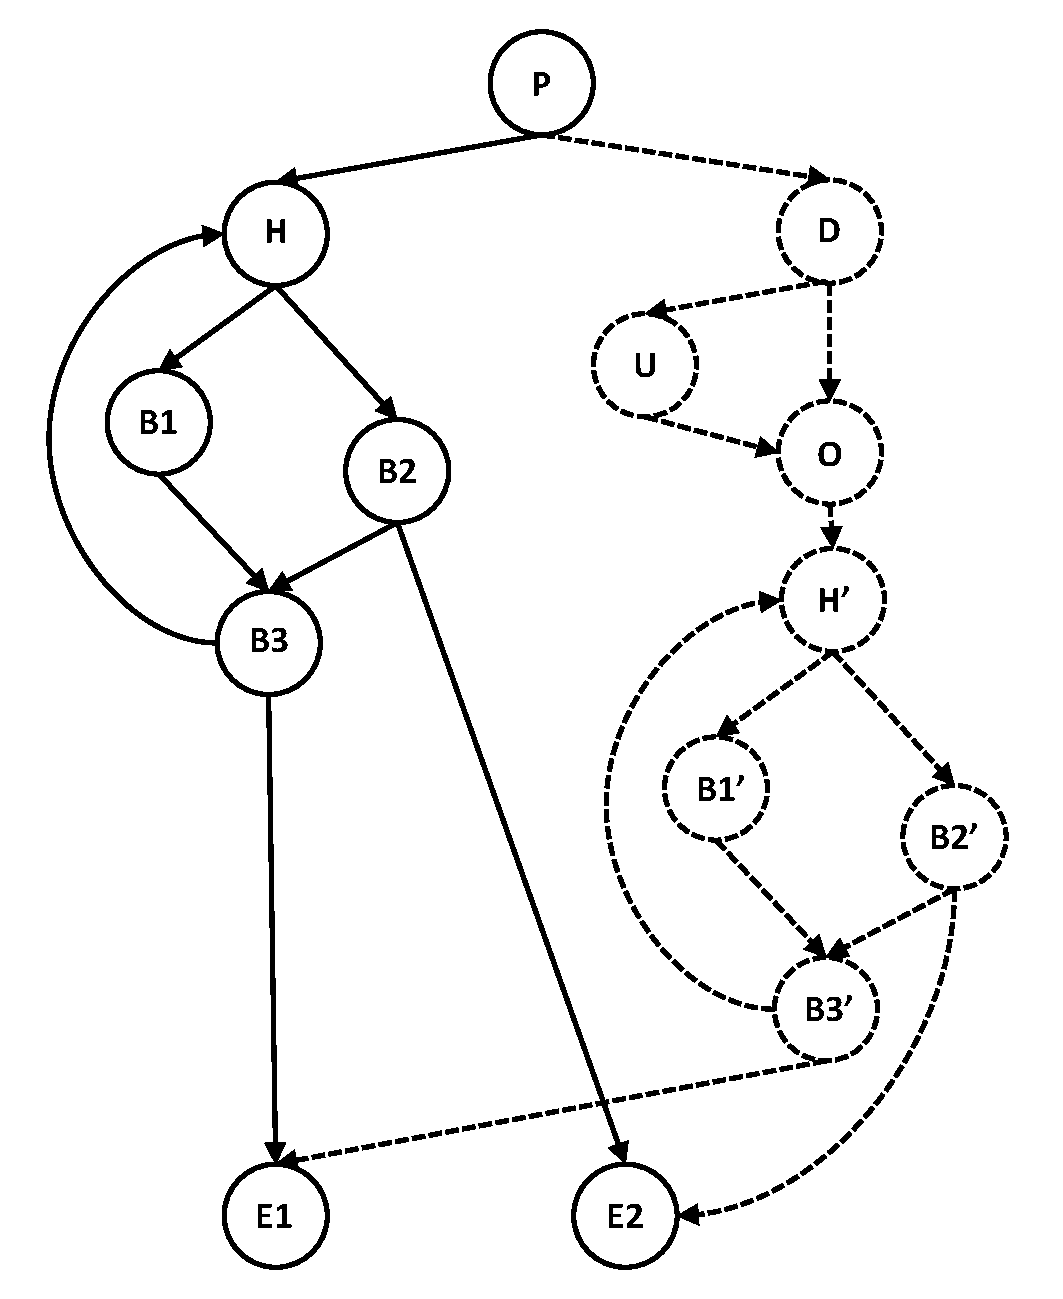
\includegraphics[width=0.7\linewidth]{figures/CL-I}
%\caption{Cross-loop Instrumentation}
%\label{fig:CL-I}
%\end{figure}

Recording values returned by every input instruction would lead to 
huge run-time overhead.
\Tool uses random sampling to reduce this overhead, which 
requires almost no changes to our redundancy 
identification algorithm discussed in Section \ref{sec:cal}.

Note that, although \Tool uses sampling, its diagnosis is still conducted
in just \textbf{one} run, with almost \textbf{no}
sacrifice to diagnosis latency or quality. This is
\textbf{different} from traditional sampling techniques
for correctness diagnosis \cite{liblit03,liblit05}, where
many more failure runs and hence longer latency
are needed once sampling is enabled.
The reason is that performance bugs have a unique repetitive nature:
a loop can cause a severe performance problem only when it 
contains many redundant iterations/instances.
Therefore, we can still recognize redundant behavior in just
\textbf{one} failure run, 
as long as the sampling is not insanely sparse
(Section \ref{sec:experiment}). 
%Another observation, which can also be demonstrated by examples shown in Figure~\ref{fig:Mozilla477564} and Figure~\ref{fig:Apache34464}, 
%is that two consecutive loop instances are good targets to compare.

%There are two possible reasons for cross-iteration redundancy. 
%The first one is loop-invariant computation, which can be identified statically, 
%and it is the target for traditional compiler optimization. 
%The second one is repetitive processed elements, like GCC\#27733 shown in Figure~\ref{fig:GCC27733}. 
%When processed elements are repetitive, the computation conducted by different iterations is exactly the same. 
%If we compare a pair of iterations, we may fail to observe redundancy. 
%For cross-iteration redundancy, we randomly sample iterations, 
%and compare distinct computation number with the total number of sampled iterations. 

For cross-iteration redundancy analysis,
we randomly decide at the
beginning of every iteration whether to track the values returned by
input instructions in this iteration.
The implementation is similar with previous sampling work 
\cite{liblit03,liblit05}.
Specifically, we create a clone of the original
loop iteration code, 
%including functions called by the loop directly or indirectly, 
and insert value-recording instructions along the
cloned copy. 
We then insert a code snippet that randomly decides to execute the
cloned copy or the original copy at the beginning of a loop iteration. 
\comment{
Two variables \texttt{CurrentID}, which is initialized as 0, 
and \texttt{NextSampleID}, which is initialized by a random integer, 
are maintained
in this code snippet. \texttt{CurrentID} is increased by 1
for each iteration. When it matches \texttt{NextSampleID}, the control
flow jumps to the value-recording clone of the loop iteration and the 
\texttt{NextSampleID} is increased by a random value. Different sampling
sparsity setting will determine the range from which the random value is
generated.
}

%\begin{figure}
%\center
%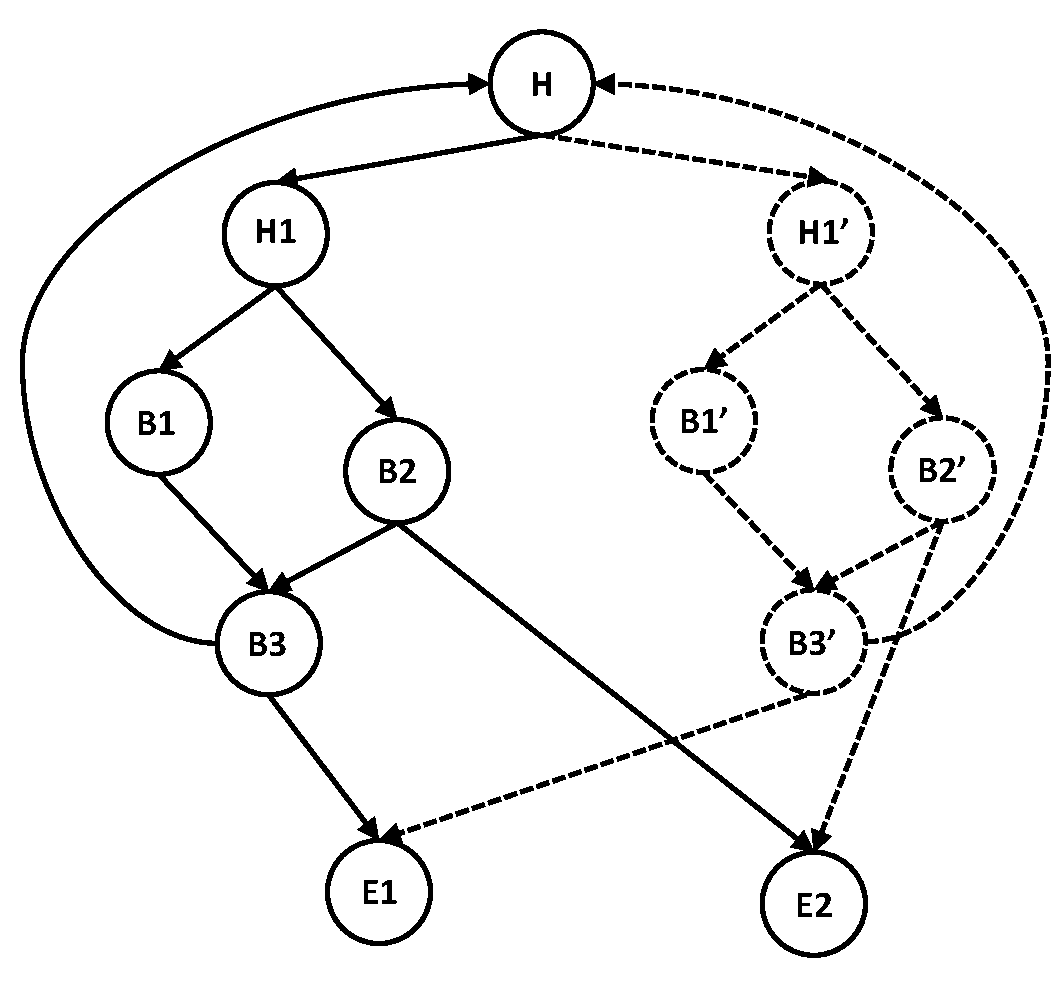
\includegraphics[width=0.7\linewidth]{figures/CI-I}
%\caption{Cross-iteration Instrumentation}
%\label{fig:CI-I}
%\end{figure}

For cross-loop redundancy analysis,
we randomly decide at the beginning
of every loop instance whether to track values for this instance. 
Since we will need to compare two consecutive loop
instances for redundancy, once we decide to sample one loop instance, we will
make sure to sample the immediate next loop instance too.
The implementation is straightforward by cloning the whole loop and making
sampling decisions in the loop pre-headers.
%; (2)
%sampling is conducted when \texttt{CurrentID} equals either
%\texttt{NextSampleID} or \texttt{NextSampleID}$+1$, with \texttt{NextSampleID}
%increased by a random value in the latter case.

%TODO
%For each monitored memmove or memcpy instruction, 
%we record its ID, the length of accessed memory, 
%and the content of the accessed memory. 



%\paragraph{Handling recursive functions}
%We also conduct sampling to our redundancy analysis for recursive functions.
%For a recursive function, we first create an instrumented clone copy of 
%the whole function body.
%We then add a sampling-control code snippet at the entry point of the function,
%where \texttt{CurrentID} and \texttt{NextSampleID} are maintained to decide
%whether to execute the original function body or the instrumented 
%value-recording clone copy.
%We also create clones for all the callee functions of the recursive function
%under study, so that the sampling decision can be correctly conducted
%throughout the call chain.

\subsubsection{Static optimization}
\label{sec:perf}

We conduct a series of static analysis to reduce the number of instructions we 
need to monitor. 

First, we avoid tracking multiple reads that we can statically 
prove to return the same value.
Since we implement \Tool in LLVM, we leverage the SSA construction and the
\textit{mem2reg} pass in LLVM to avoid unnecessary tracking of
stack variables.
For example, the read of \texttt{max} on line 10 of 
Figure \ref{fig:Apache34464} is an \textit{input} instruction of the 
\texttt{while} loop on the same line. LLVM identifies it as a loop invariant
and lifts the read of \texttt{max}
out of the loop. Consequently, \Tool only records
its value once during each loop, instead of each iteration.
LLVM is conservative in lifting heap/global variables out of
a loop.
%, for fear of changing the location of potential exceptions.
\Tool conducts a best-effort
loop invariant analysis for heap/global variables.
For example, \Tool identifies that the values of
\texttt{aNode->localName} and \texttt{aNode->namespaceURI} do not change
throughout one loop instance
in Figure~\ref{fig:Mozilla477564}, and hence only traces them once
outside the loop.

\comment{
This analysis is sound but not complete.
\Tool may miss some loop invariants. For in-house debugging, since we know
the problem-triggering inputs do not lead to exceptions, this optimization
is safe. For production-run usage, users can turn off this heap/global
variable related optimization.
}

Second, we leverage the scalar evolution (SE) analysis in LLVM to remove the 
monitoring to some loop-induction related variables.
SE analysis can tell which variables are
loop-induction variables (e.g., \texttt{i} on line 10
of Figure~\ref{fig:Apache34464}) and what are their strides. 
In cross-iteration redundancy checking,
if a loop iteration's input set contains a loop-induction
variable, we know different iterations' inputs would be different and 
hence conclude that there is no redundancy without
run-time analysis.
In cross-loop redundancy checking,
when the address of a read is a loop induction variable, such as
\texttt{source[i]} on line 10 of Figure~\ref{fig:Apache34464},
we only record the address range at run time,
instead of every value returned by the memory read.
This optimization could lead to false positives ---
different loop instances may work on variables read from
similar memory locations but with different values.
We did not encounter such false positives in our experiments.


\subsection{Fix Strategy Recommendation}
\label{sec:redundant_fix}

\Tool suggests a fix strategy for each inefficient loop based on the
inefficiency category. Making this suggestion is straightforward for
most categories, and requires a small amount of extra
analysis occasionally. \Tool also
provides related information for carrying out the suggested fix strategy. 

Once a loop is identified as \emph{resultless}, \Tool will suggest
the loop to be deleted in case of 0$^*$,
conditionally skipped in case of [0$|$1]*, or a
data-structure change in case of 0*1?.
\Tool also reports side-effect instructions 
and what percentage of loop iterations executes each such instruction,
helping developers refactor the loop or change data structures. 

When a loop is identified as \emph{redundant}, \Tool conducts
extra analysis to
decide whether batching or memoization should be used. 
For cross-iteration redundancy, \Tool suggests batching 
I/O operations.
when the only side effect of a loop is from I/O operations
and the same statement(s) is executed in every iteration.
Otherwise, \Tool suggests memoization, and reports
input instructions that lead to redundant computation and redundancy rate.

For cross-loop redundancy, whether to use memoization or batching often
depends on which strategy is cheaper.
\Tool uses a simple
heuristic. If 
the side effect of each loop instance is to update 
a constant number of memory locations, like the 
buggy loop in Figure~\ref{fig:Mozilla477564} and Figure~\ref{fig:Apache34464}, 
we recommend memoization. If the side effect is to update
a sequence of memory locations, with the number of locations increasing
with the workload, memoization is unlikely to save much and
hence batching is suggested.
\Tool will also report
the memory reads that return the same values
again and again, which can help decide what to memoize.

\comment{
%%if side effect of the loop is to define several scalar value used outside the loop, we recommend memoization.
%%if side effect is to write to distinct memory address or conduct system call, 
%%we recommend batch

%It is easy to lift read from local variable outside the loop. 
%Compiler is conservative to move read, which may cause exception, outside the loop.
%I think this part of analysis is to prune memory read which is invariant, but unsafe to be moved out by compiler. 
%llvm is very conservative to move memory read from array/structure/global variable/heap variable
%outside the loop.
%what we do is if the read address is loop invariant, and there are no other write possibly 
%write to the same place, we will not record the memory read.

%ANSWER:
%while(i=lower[j]; a[i]<100 & i<upper[j]; i++); 
%The memory read upper[j] is conducted in each iteration.
%The read address upper+j is loop-invariant. If there is not write to the same
%address, the read is also loop-invariant, and we do not need to record the memory read.
%we conduct alias analysis, and analysis whether there are memory writes, whose
%address may/must alias to the read address. 

%induction variables are not always identified as source instructions.
%it could be possible that side-effect instructions do not depend on induction variables.
%for example, side-effect instruction may only depend on array content, and array index 
%will not be source instructions

%TODO: Linhai, I find it hard to believe that consider "there will not be
%cross-iteration redundancy simply because induction variable is in the 
%dependent set. Really? The input workload itself could be repetitive, and hence
%could still deserve monitoring, right? 
%


%ANSWER: this is true according to how we calculate cross-iteration redundancy.
%We only consider iteration from the same loop instance.
%induction variable will be changed in each iteration by a fix constant, so
%the value of induction variable will be different from each other in each iteration of the same loop instance. 
%The case you mention is 
%for(i=0; i < 10; i ++) {
%  c = A[i]; 
%   ...   // all other computation only depend on c        
% }
%Our dependence analysis will report the memory read A[i] as dependent value, not i.
%If the content of A is repetitive, we will identify cross-iteration redundancy.
 
%For cross-iteration instrumentation, we use scalar evolution analysis to identify 
%whether there are induction variables in the dependent value set. 
%A induction variable will be increased or decreased by a fix amount in each loop iteration. 
%If there are induction variable inside the dependent value set, 
%we know that there will not be cross-iteration redundancy. 

%TODO Linhai, I don't understand your original text. The address is 
%source+i; loop induction variable is i. What do you mean by "the read address
%is an induction variable"? Please rewrite.

%ANSWER
%Shan, both source + i and i are induction variables, because both of them 
%will be added by 1 in each iteration. The only difference between these two 
%are their initial values.
%For cross-loop redundant bugs, we also rely on scalar evolution analysis to identify whether the read address
%is an induction variable for each monitored read instruction. 

\comment{
We consider two types of dependence, control dependence and RAW data dependence. 
We build control dependence graph according to the algorithm discussed in~\cite{controldep}. 
If block A is one of ancestors of block B on the control dependence graph, 
we consider all instructions in block B control depend on the branch condition in block A. 
Data dependence is mainly calculated based on instructions' operands. 
We define several types of instrumentation sites. 
The inputs of our dependence analysis are instructions, 
and the output of our dependence analysis is a set of dependent values, 
including instrumentation sites and constant values. 

Before calculating dependence inside the monitored loop, 
we conduct inter-procedural dependence analysis for each function directly called by the loop. 
The formal parameters of each direct callee, memory instructions, 
including load, memcpy, and memmove, 
whose source is not from local structures or arrays, 
and return values of library function calls are instrumentation sites. 
During calculating dependence, 
we consider formal parameter data depend on all real parameter, 
the return value of each call site data depend on return inside the callee function, 
and all instructions inside one callee functions inherit control dependence of all its call site. 

If a direct callee from the monitored loop does not contain recursive function calls, 
we use a three-stage method to solve the infeasible path problem. 
Assume function A is called inside the monitored loop, function A will call function B, 
and function B will call function C. 
We will have a call tree A $\rightarrow$ B $\rightarrow$ C. 
This call tree does not have recursive function calls, so our three-stage method can apply to this case. 
At the first stage, we conduct intra-procedural dependence analysis for each function.  
We consider return values of all call sites as instrumentation sites. 
For example, we consider both the return value of B in A and the return value of C in B as instrumentation sites. 
At the second stage, we process each function bottom-up on the call tree. 
For each call site inside a function, we calculate 
how the return value depend on real parameters based on dependence information inside the callee.
Back to our example, we will process the three functions in order C, B, and A.
When processing function B, we calculate the dependence for the return value of function C 
based on the dependence information inside C and the real parameters of the call site.
At the last stage, we process each function top-down on call tree, 
and calculate dependence for instruction inside a callee function based on information from all its call site. 
At this stage, we will process the three function in the order A, B, and C. 
We update dependence information inside function B, according to control dependence and real parameters of its call site in A. 

We design a Gen-Kill based intra-procedural analysis to 
calculate which previous writes a memory read from local structures and arrays depends on. 
The basic idea is that a memory write will kill all previous writes whose destination address it can cover, 
and the memory write will generate a new write to its destination address. 
Each memory read depends on previous writes whose destination addresses overlap with its source address. 

For the monitored loop, we calculate dependent values for all site-effect instructions, 
including side-effect instructions inside the loop and side-effect instructions inside the callees. 
For cross-loop dependence analysis, instrumentation sites include values defined outside the loop, 
memory reads inside the loop, memory reads not from local structure and arrays inside callees, 
and return values of library function calls. 
For cross-iteration dependent analysis, instrumented sites also include value defined in previous iterations. 
For example, the instruction defining the value of \texttt{i} is the only side-effect instruction 
inside the loop at line 12 in Figure~\ref{fig:Apache34464}. 
After running cross-loop dependence analysis, the dependent values include 
memory read \texttt{source[i]} inside the loop, 
and three values defined outside the loop, 
which represent the initial value of \texttt{i}, the value of \texttt{max} and \texttt{first} respectively. 
After running cross-iteration dependence analysis, 
the dependent value include value \texttt{i} defined in previous iteration, 
memory read \texttt{source[i]}, 
and two values defined outside the loop (\texttt{max} and \texttt{first}).  

}

}
